\chapter{Prometheus}


Prometheus是一个开源的完整监控解决方案,其对传统监控系统的测试和告警模型进行了彻底的颠覆,形成了基于中央化的规则计算、统一分析和告警的新模型。

\begin{figure}[H]
    \centering
    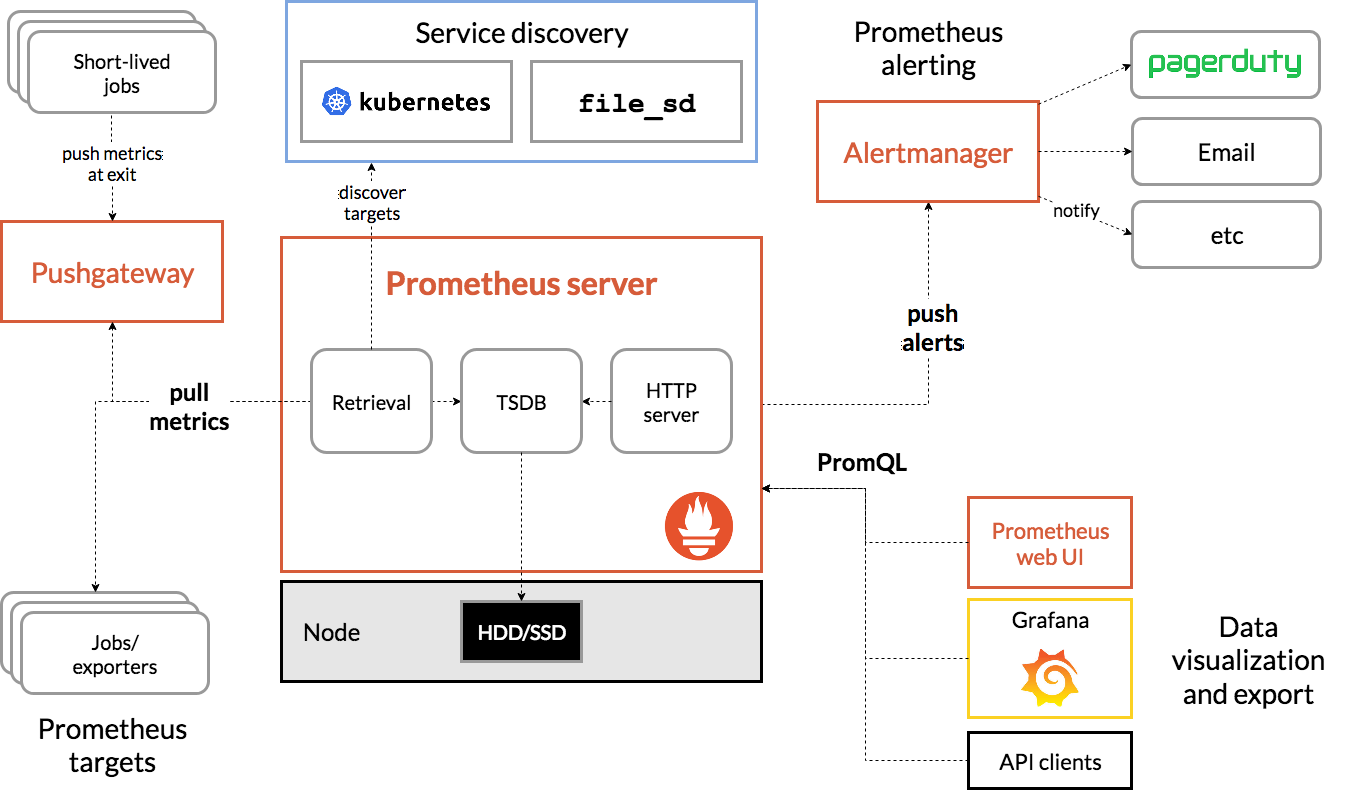
\includegraphics[width=1\textwidth]{prometheus/architecture.png}
    \caption{Architecture}
\end{figure}


其优点

\begin{itemize}
    \item 易于管理
    \item 监控服务的内部运行状态
    \item 强大的数据模型
    \item 强大的查询语言PromQL
    \item 高效
    \item 可扩展
    \item 易于集成
    \item 可视化
    \item 开放性
\end{itemize}

\subsection{安装}

二进制包安装


\href{https://prometheus.io/download/}{https://prometheus.io/download/} 下载二进制包解压运行即可

Docker

\href{https://hub.docker.com/r/prom/prometheus}{https://hub.docker.com/r/prom/prometheus}


\subsection{数据模型}

按照相同时序(相同的名字和标签),以时间维度存储连续的数据的集合。


格式

\begin{lstlisting}[language=shell]
<metric name>{<label name>=<label value>, ...}
\end{lstlisting}

\subsubsection{时序类型}

Prometheus 时序数据分为 Counter, Gauge, Histogram, Summary 四种类型。

Counter

Counter 表示收集的数据是按照某个趋势(增加/减少)一直变化的,我们往往用它记录服务请求总量、错误总数等。

\begin{lstlisting}[language=shell]
prometheus_http_requests_total{code="200",group="beijing",handler="/metrics",instance="127.0.0.1:9090",job="prometheus-server",monitor="prometheus"}

100
\end{lstlisting}

Gauge

Gauge 表示搜集的数据是一个瞬时的值,与时间没有关系,可以任意变高变低,往往可以用来记录内存使用率、磁盘使用率等。

Histogram

Histogram 由 \<basename\>_bucket{le="\<upper inclusive bound\>"},\<basename\>_bucket{le="+Inf"}, \<basename\>_sum,\<basename\>_count 组成,主要用于表示一段时间范围内对数据进行采样(通常是请求持续时间或响应大小),并能够对其指定区间以及总数进行统计,通常它采集的数据展示为直方图。


Summary

Summary 和 Histogram 类似,由 \<basename\>{quantile="<φ>"},\<basename\>_sum,\<basename\>_count 组成,主要用于表示一段时间内数据采样结果(通常是请求持续时间或响应大小),它直接存储了 quantile 数据,而不是根据统计区间计算出来的。




以`prometheus_http_requests_total`为例

\begin{lstlisting}[language=shell]
    prometheus_http_requests_total  # 等同于prometheus_http_requests_total{}
\end{lstlisting}

该表达式会返回指标名称为prometheus_http_requests_total的所有时间序列


支持两种匹配模式

* 完全匹配

    - 通过使用label=value可以选择那些标签满足表达式定义的时间序列;
    - 反之使用label!=value则可以根据标签匹配排除时间序列;


* 正则匹配

支持使用正则表达式作为匹配条件,关键字为`~`。多个表达式之间使用`|`进行分离

    - 使用label=~regx表示选择那些标签符合正则表达式定义的时间序列;
    - 反之使用label!~regx进行排除;


范围查询

[]


\subsection{操作符}



\subsubsection{聚合操作}

内置的聚合操作符是作用于瞬时向量。可以将瞬时表达式返回的样本数据进行聚合,形成一个具有较少样本值的新的时间序列。

\begin{itemize}
    \item sum(求和)
    \item  min(最小值)
    \item  max(最大值)
    \item  avg(平均值)
    \item  stddev(标准差)
    \item  stdvar(标准差异)
    \item  count(计数)
    \item  count_values(对value进行计数)
    \item  bottomk(样本值最小的K个元素)
    \item  topk(样本值最大的K个元素)
    \item  quantile(分布统计)
\end{itemize}

通过without或者by子句来保留不同的维度。

\begin{lstlisting}[language=shell]

    [aggr-op]([parameter,] <vector expression>) [without|by(label list)]

\end{lstlisting}

其中只有`count_values`、`quantile`、`topk`、`bottomk`支持参数。

`without` 用于从计算结果中移除列举的标签,而保留其他标签。

`by` 结果向量中只保留列出的标签,其余标签则移除。







